\documentclass[12pt]{elsart}
\usepackage{amsmath}
\usepackage{amssymb}
\usepackage{program}
\usepackage{graphicx}
\usepackage[table]{xcolor}% http://ctan.org/pkg/xcolor
\newcommand{\field}[1]{\mathbb{#1}}

\usepackage{algorithm}
\usepackage{algpseudocode}

%%%%%%%%%%%%%%%%%%%%%%%%%%%%%%%%%%%%%%%%%Space to make more readable!
%\vspace{10 mm}
%%%%%%%%%%%%%%%%%%%%%%%%%%%%%%%%%%%%%%%%%Take out later!

\begin{document}
Bryan Burkhardt - XMV643\\
CS3343 Section 01\\
22 Oct 2017\\

\pagestyle{empty}

\begin{center}
\Large  CS3343 Analysis of Algorithms Fall 2017 \\
\large {\bf Homework 5}\\
\normalsize Due 10/22/17 before 11:59pm (Central Time)
\end{center}

{\bf 1.  Hash Table Probabilities (3 points)}

\begin{enumerate}
   \item (1 point) Suppose $2$ keys are inserted into an empty hash table with $m$ slots. Assuming
simple uniform hashing, what is the probability of:
\begin{enumerate}
   \item exactly $0$ collisions occurring\\\\
	\boxed{\frac{m-1}{m}}\\
	Because if we insert key 1 into a slot. The total empty slots remaining $= m-1$. Thus, there are $\frac{m-1}{m}$ slots for key 2 to be inserted.\\
   \item exactly $1$ collisions occurring\\\\
	\boxed{\frac{1}{m}}\\
	Because if we insert key 1 into a slot, the total filled slots $= \frac{1}{m}$. Thus, there is a $\frac{1}{m}$ chance that key 2 will collide.\\
\end{enumerate}

   \item (2 points) Suppose $3$ keys are inserted into an empty hash table with $m$ slots. Assuming
simple uniform hashing, what is the probability of:
\begin{enumerate}
   \item exactly $0$ collisions occurring\\\\
	\boxed{$($\frac{m-1}{m})(\frac{m-2}{m})}\\
	We start by inserting key 1 which has no chance of colliding which also gives us $m-1$ empty slots remaining. The chance of key 2 colliding with key 1 is $\frac{m-1}{m}$. Next, key 2 is inserted without colliding, giving us $\frac{m-2}{m}$ empty slots remaining. The chance of key 3 colliding with key 1 or key 2 is the product of the two previous values.\\
\newpage
   \item exactly $1$ collisions occurring\\\\
	\boxed{$($3)(\frac{m-1}{m})(\frac{1}{m})}\\\\
	{\bf Scenario 1: Key 1 and Key 2 don't collide, Key 3 does.}\\
	 Probability of key 1 colliding $=\frac{m}{m}$. Probability of key 2 not colliding with key 1 $=\frac{m-1}{m}$. Probability of key 3 colliding with key 1 or 2 $=\frac{2}{m}$. Therefore, the probability for scenario 1 $=(\frac{m-1}{m})(\frac{2}{m})$\\\\
	{\bf Scenario 2: key 1 and key 2 collide, key 3 does not.}\\
	Proability of key 1 not colliding $=\frac{m}{m}$. Probability of key 2 colliding with key 1 $=\frac{1}{m}$. Probability of key 3 not colliding $=\frac{m-1}{m}$. Therefore, the probability of scenario 2 $=(\frac{1}{m})(\frac{m-1}{m})$.\\\\
	Scenario 1 $+$ Scenario 2 $=$ the boxed answer above.\\

   \item exactly $2$ collisions occurring\\\\
	\boxed{\frac{1}{m^2}}\\
	Probability of key 1 colliding $=\frac{m}{m}$. Probability of key 2 colliding with key 1 $=\frac{1}{m}$. Probability of key 3 colliding with key 1 and 2 $=\frac{1}{m}$. We then take the product of the two probabilities and get the answer boxed above.
\end{enumerate}

\end{enumerate}


{\bf 2.  Red-Black Trees (2 points)}

\begin{enumerate}
\item Company X has created a new variant on red-black trees which also uses blue as a color for the nodes.  They call these ``red-black-blue trees".  Below are the new rules for these trees:\\

\begin{itemize}
   \item Every node is red, blue, or black.
   \item  The root is black.
   \item Every leaf (NIL) is black.
   \item If a node is red, then both its children are black.
   \item If a node is blue, then both its children are red or black.
   \item For each node, all simple paths from the node to descendant leaves contain the
same number of black nodes.\\
\end{itemize}
\newpage
\begin{enumerate}
   \item (2 points) In class we found that the height, $h$, of a red-black tree is $\leq 2\log_2(n+1)$ (where $n$ is the number of keys).  Find and prove that a similar bound on height of the red-black-blue trees.
\\\\(Hint: You can use the same approach as we did to show\\ $h \leq 2\log_2(n+1)$).\\\\
	{\bf Answer:}\\
	Worst case scenario, our tree goes $black \rightarrow blue \rightarrow red \rightarrow black \rightarrow blue \rightarrow red \rightarrow \ldots$\\
	Therefore, our compression factor would be $\frac{h}{3}$\\
	so,\\ 
	$(n+1) \geq {2^h}^\prime$\\
	$\log_2{(n+1)} \geq h^\prime \geq \frac{h}{3}$\\
	$\boxed{\Rightarrow h \lt 3\log_2{(n+1)}}$\\

   \item (0 points - just for fun) Adding an additional color didn't seem to improve our bound on $h$ (i.e., 3 colors allows the tree to become more unbalanced than with 2 colors).    What benefit might we get from the extra color?
\end{enumerate}

\end{enumerate}



{\bf 3.  B-trees (4 points)}

\begin{enumerate}
   \item (2 points) Show the results of inserting the keys\\\\
$E,F,G,U,V,W,H$\\\\
in order into the B-tree shown below.  Assume this B-tree has minimum degree $k=2$. Draw only the configurations
of the tree just before some node(s) must split, and also draw the final configuration.

\vspace{-1.5mm}
\begin{figure}[h]
	\centering 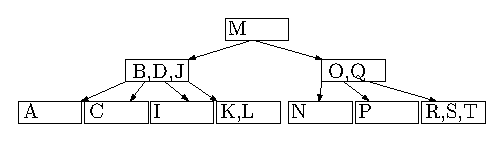
\includegraphics[width=0.7\textwidth]{BTreeProblem-01}
\end{figure}
\vspace{-1.5mm}
\newpage
	
	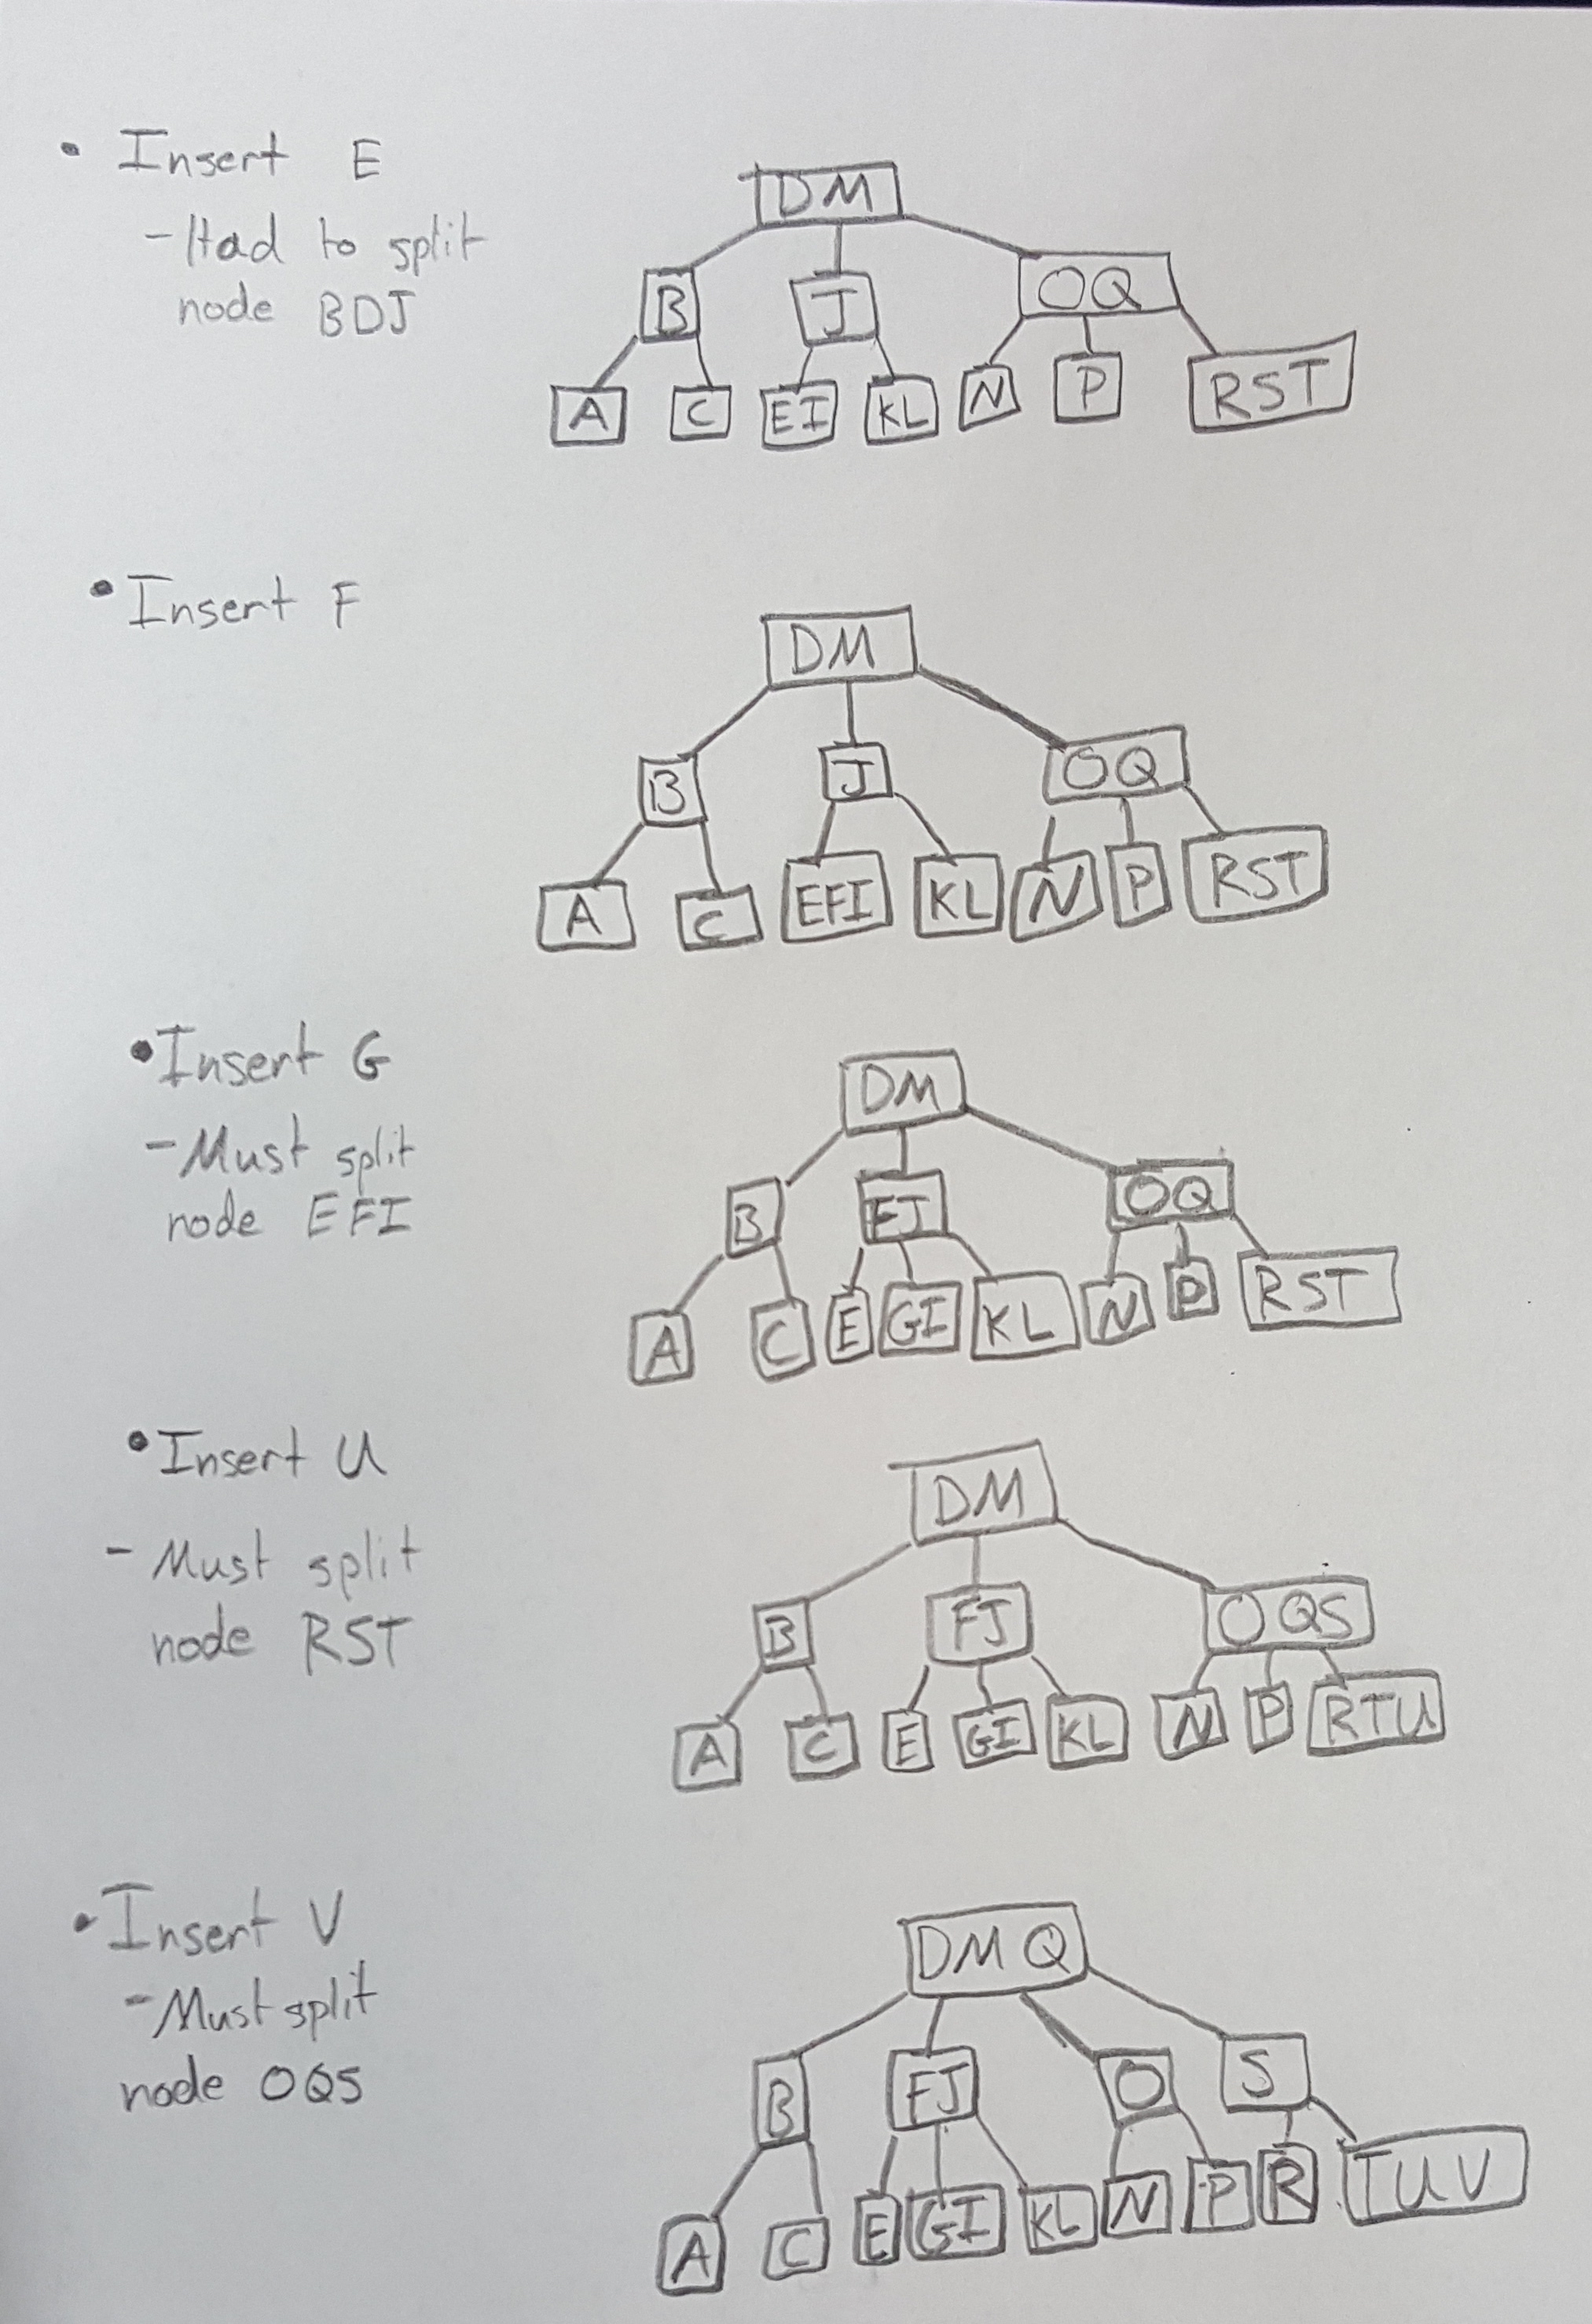
\includegraphics[scale=0.12]{part1.jpg}\\
	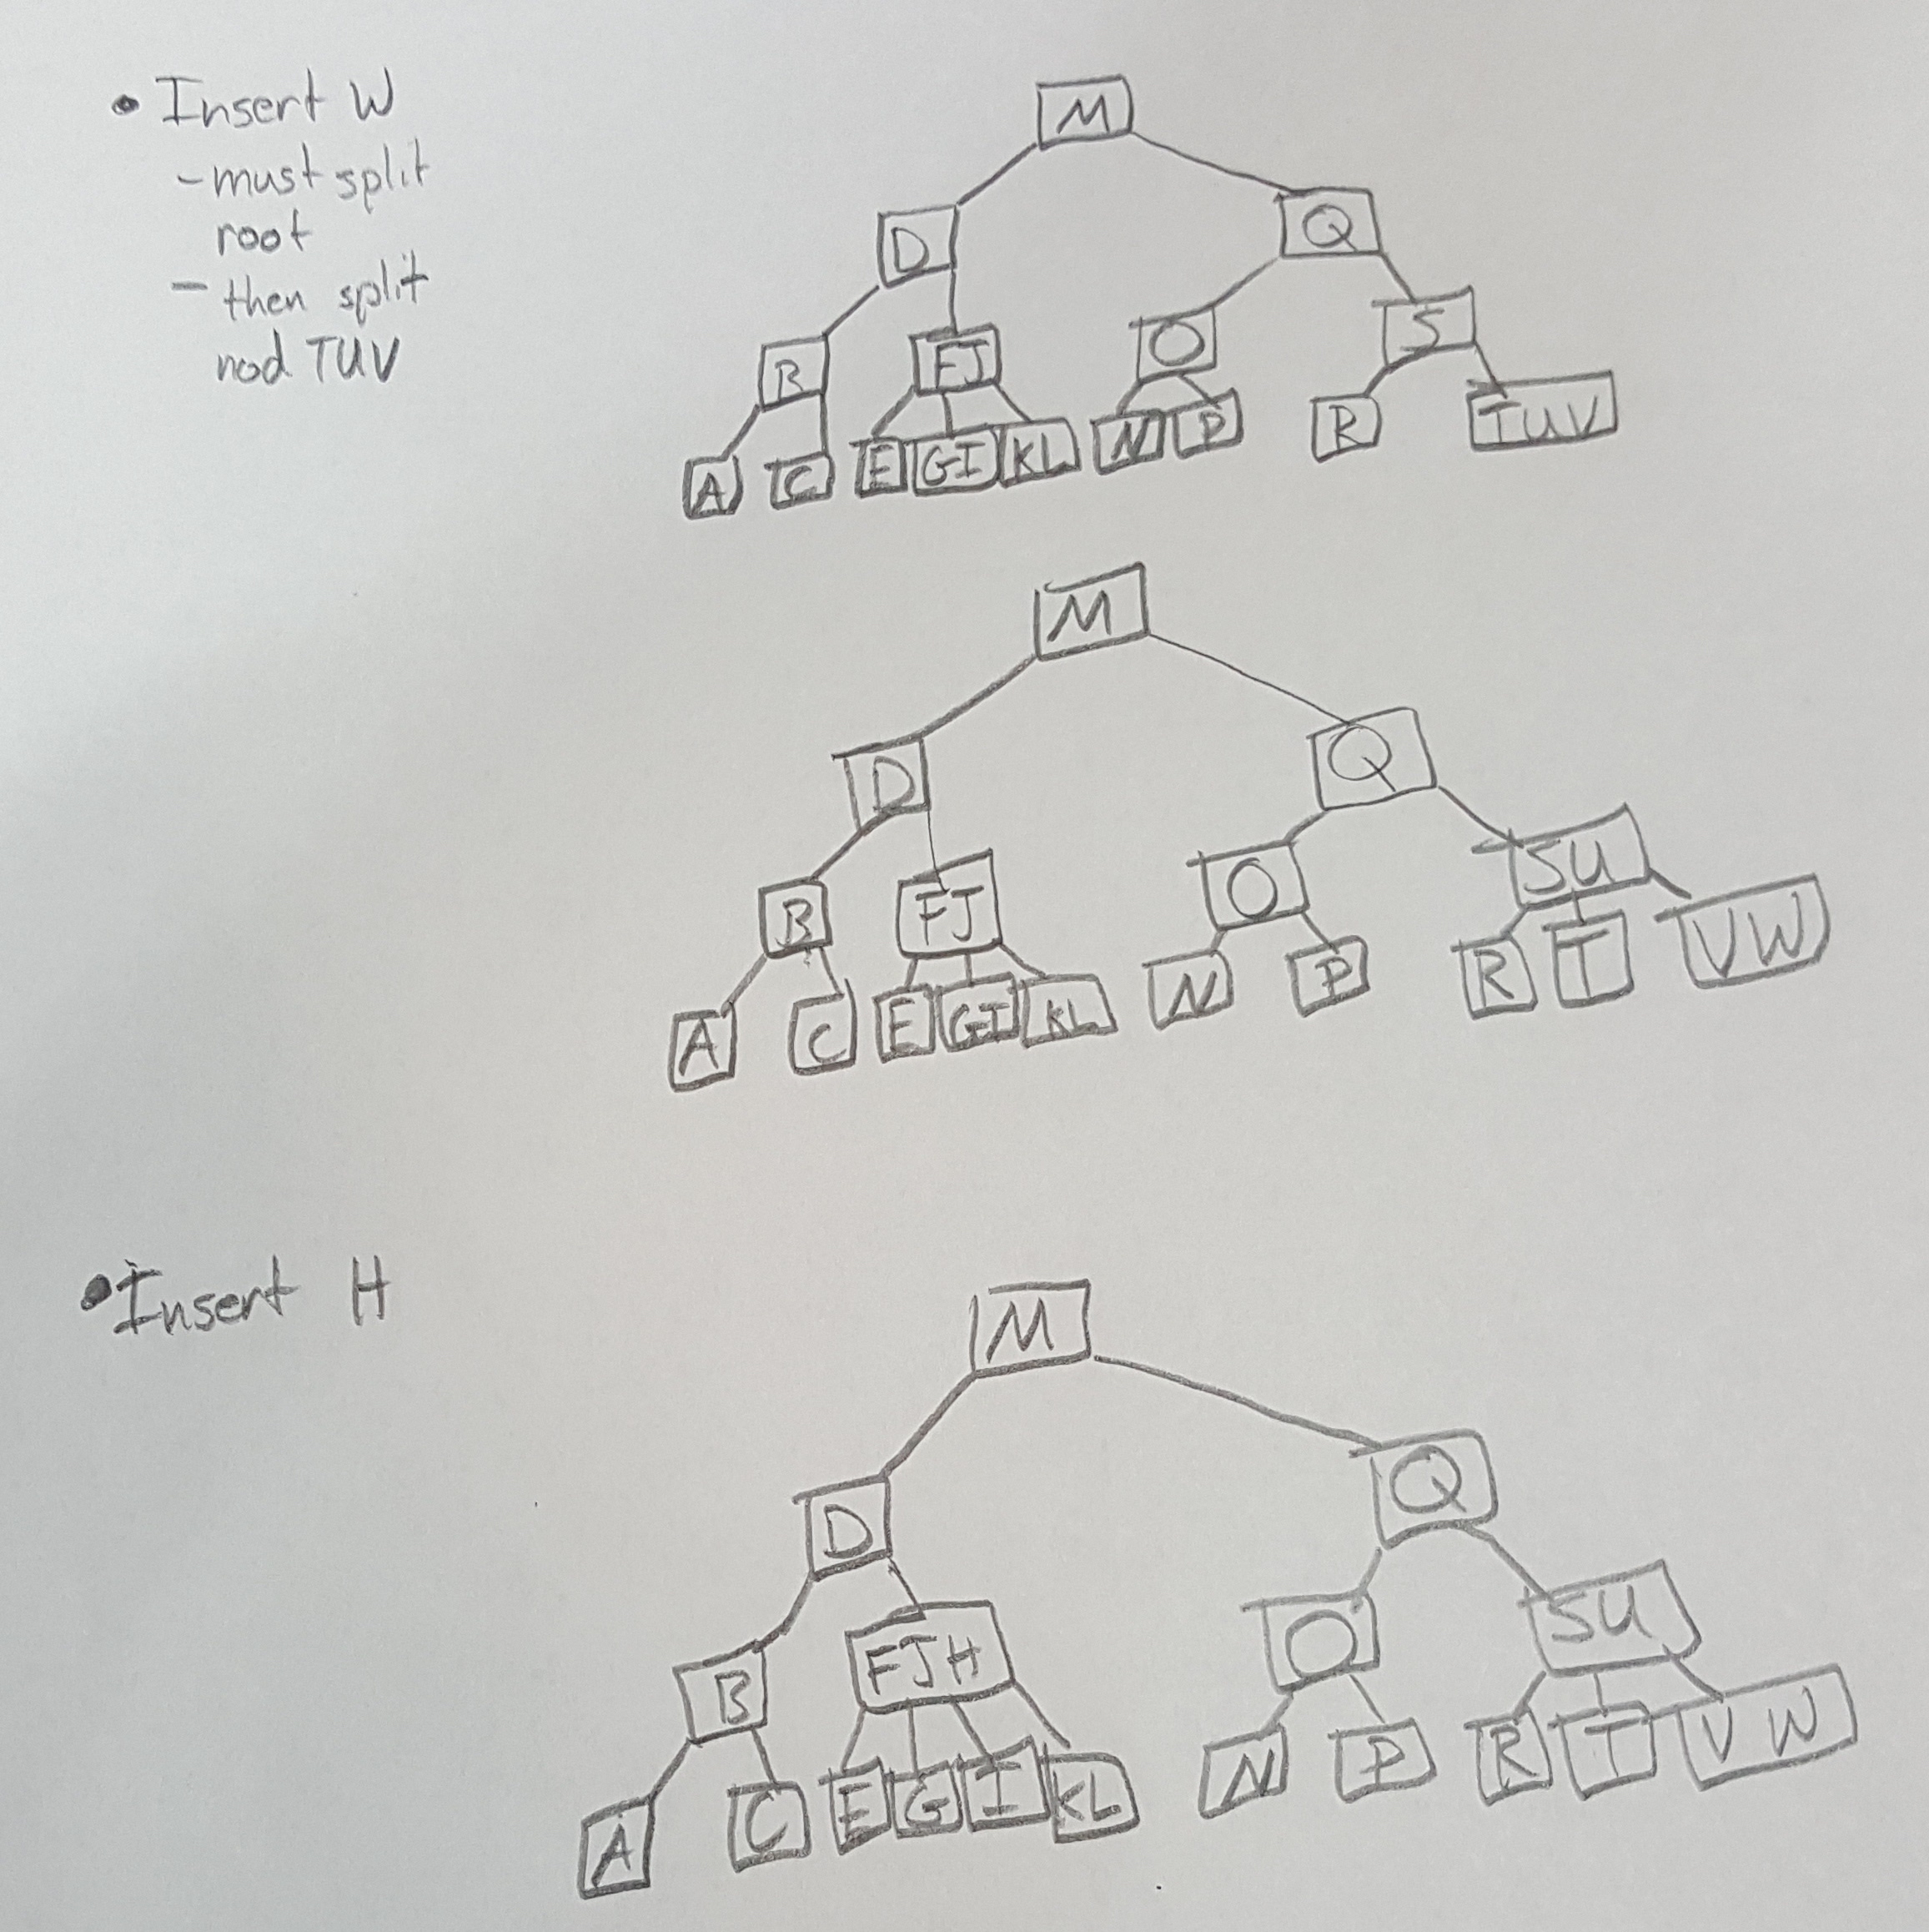
\includegraphics[scale=0.12]{part2.jpg}
\newpage
   \item (2 points) Suppose you have a B-tree of height $h$ and minimum degree $k$. What is the largest number of keys that can be stored in such a B-tree?  Prove that your answer is correct.
\\\\(Hint: Your answer should depend on $k$ and $h$. This is similar to \\theorem we proved in the B-tree notes).\\\\
	{\bf Answer:}
	Say we have a tree of $h=3$ and $k=2$. At level 1, our root would have a maximum of 3 keys. Level 2, would have 4 children, each with 3 keys, $(4)(3)=12$ keys. Level 3 would have 16 children, each with 3 keys, $(16)(3)=48$  keys. $48+12+3=63$ keys total.\\\\
	$\sum\limits_{i=0}^{h-1}h(2k)^i = h\sum\limits_{i=0}^{h-1}(2k)^i = \boxed{(h)$($\frac{(2k)^h-1}{2k-1})}$\\
	$(3)$($\frac{(2(2))^3-1}{2(2)-1}) = 63$\\
\end{enumerate}
\newpage
{\bf 4.  Choose Function (4 points)}

Given $n$ and $k$ with $n \geq k \geq 0$, we want to compute the choose function ${n \choose k}$ using the following recurrence:

\hspace*{0.5cm} Base Cases: ${n \choose 0}=1$ and ${n \choose n}=1$, for $n\geq 0$\\
\hspace*{0.5cm} Recursive Case: ${n \choose k} = {n-1 \choose k-1} + {n-1 \choose k}$, for $n>k>0$

   \begin{enumerate}
      \item (1 point) Compute ${5 \choose 3}$ using the above recurrence.\\\\
	${5 \choose 3}$\\
	$ = {4 \choose 2}+{4 \choose 3}$\\
	$= [{3 \choose 1}+{3 \choose 2}] + [{3 \choose 2}+{3 \choose 3}]$\\
	$=[{2 \choose 0}+{2 \choose 1}]+[{2 \choose 1}+{2 \choose 2}]+[{2 \choose 1}+{2 \choose 2}]+[1]$\\
	$=[1]+[{1 \choose 0}+{1 \choose 1}]+{1 \choose 0}+{2 \choose 0}]+[1]+[{1 \choose 0}+{2 \choose 0}]+[1]+[1]$\\
	$=1+1+1+1+1+1+1+1+1+1$\\
	$=\boxed{10}$\\
      \item (2 points) Give pseudo-code for a {\bf bottom-up} dynamic programming algorithm to compute ${n \choose k}$ using the above recurrence.
	\begin{algorithm}
	\caption{choose(int n, int k)}
		\begin{algorithmic}
		\If{(k==0 or n++k)}
			\State return 1;
		\EndIf
		\For{$i=n$ to $1$}
			\For{$j=k$ to $0$}
				\State $T[n][k] = T[n-1][k-1]+T[n-1][k]$
			\EndFor
		\EndFor
		\end{algorithmic}
	\end{algorithm}
\newpage
      \item (1 point) Show the dynamic programming table your algorithm creates for ${5 \choose 3}$.

\begin{tabular}{ l||p{0.1\linewidth}|p{0.1\linewidth}|p{0.1\linewidth}|p{0.1\linewidth}|}
   & 0 & 1 & 2 & 3  \\
  \hline
  \hline
   0& 1 & \cellcolor{black!100} & \cellcolor{black!100}  & \cellcolor{black!100}\\
  \hline
   1& 1 & 1 & \cellcolor{black!100} & \cellcolor{black!100}\\
  \hline
   2& 1 & 2 & 1 & \cellcolor{black!100}\\
  \hline
   3& 1 & 3 & 3 & 1\\
  \hline
   4& 1 & 4 & 6 &4\\
  \hline
   5& 1 & 5 & 10 &10\\
  \hline
\end{tabular}
   \end{enumerate}

\end{document}